% Options for packages loaded elsewhere
\PassOptionsToPackage{unicode}{hyperref}
\PassOptionsToPackage{hyphens}{url}
%
\documentclass[
  english,
  man,floatsintext]{apa6}
\usepackage{amsmath,amssymb}
\usepackage{lmodern}
\usepackage{iftex}
\ifPDFTeX
  \usepackage[T1]{fontenc}
  \usepackage[utf8]{inputenc}
  \usepackage{textcomp} % provide euro and other symbols
\else % if luatex or xetex
  \usepackage{unicode-math}
  \defaultfontfeatures{Scale=MatchLowercase}
  \defaultfontfeatures[\rmfamily]{Ligatures=TeX,Scale=1}
\fi
% Use upquote if available, for straight quotes in verbatim environments
\IfFileExists{upquote.sty}{\usepackage{upquote}}{}
\IfFileExists{microtype.sty}{% use microtype if available
  \usepackage[]{microtype}
  \UseMicrotypeSet[protrusion]{basicmath} % disable protrusion for tt fonts
}{}
\makeatletter
\@ifundefined{KOMAClassName}{% if non-KOMA class
  \IfFileExists{parskip.sty}{%
    \usepackage{parskip}
  }{% else
    \setlength{\parindent}{0pt}
    \setlength{\parskip}{6pt plus 2pt minus 1pt}}
}{% if KOMA class
  \KOMAoptions{parskip=half}}
\makeatother
\usepackage{xcolor}
\IfFileExists{xurl.sty}{\usepackage{xurl}}{} % add URL line breaks if available
\IfFileExists{bookmark.sty}{\usepackage{bookmark}}{\usepackage{hyperref}}
\hypersetup{
  pdftitle={It's Time To Abandon the Cross-Lagged Panel Model},
  pdfauthor={Richard E. Lucas1},
  pdflang={en-EN},
  pdfkeywords={cross-lagged panel model, longitudinal, structural equation modeling},
  hidelinks,
  pdfcreator={LaTeX via pandoc}}
\urlstyle{same} % disable monospaced font for URLs
\usepackage{graphicx}
\makeatletter
\def\maxwidth{\ifdim\Gin@nat@width>\linewidth\linewidth\else\Gin@nat@width\fi}
\def\maxheight{\ifdim\Gin@nat@height>\textheight\textheight\else\Gin@nat@height\fi}
\makeatother
% Scale images if necessary, so that they will not overflow the page
% margins by default, and it is still possible to overwrite the defaults
% using explicit options in \includegraphics[width, height, ...]{}
\setkeys{Gin}{width=\maxwidth,height=\maxheight,keepaspectratio}
% Set default figure placement to htbp
\makeatletter
\def\fps@figure{htbp}
\makeatother
\setlength{\emergencystretch}{3em} % prevent overfull lines
\providecommand{\tightlist}{%
  \setlength{\itemsep}{0pt}\setlength{\parskip}{0pt}}
\setcounter{secnumdepth}{-\maxdimen} % remove section numbering
% Make \paragraph and \subparagraph free-standing
\ifx\paragraph\undefined\else
  \let\oldparagraph\paragraph
  \renewcommand{\paragraph}[1]{\oldparagraph{#1}\mbox{}}
\fi
\ifx\subparagraph\undefined\else
  \let\oldsubparagraph\subparagraph
  \renewcommand{\subparagraph}[1]{\oldsubparagraph{#1}\mbox{}}
\fi
\newlength{\cslhangindent}
\setlength{\cslhangindent}{1.5em}
\newlength{\csllabelwidth}
\setlength{\csllabelwidth}{3em}
\newlength{\cslentryspacingunit} % times entry-spacing
\setlength{\cslentryspacingunit}{\parskip}
\newenvironment{CSLReferences}[2] % #1 hanging-ident, #2 entry spacing
 {% don't indent paragraphs
  \setlength{\parindent}{0pt}
  % turn on hanging indent if param 1 is 1
  \ifodd #1
  \let\oldpar\par
  \def\par{\hangindent=\cslhangindent\oldpar}
  \fi
  % set entry spacing
  \setlength{\parskip}{#2\cslentryspacingunit}
 }%
 {}
\usepackage{calc}
\newcommand{\CSLBlock}[1]{#1\hfill\break}
\newcommand{\CSLLeftMargin}[1]{\parbox[t]{\csllabelwidth}{#1}}
\newcommand{\CSLRightInline}[1]{\parbox[t]{\linewidth - \csllabelwidth}{#1}\break}
\newcommand{\CSLIndent}[1]{\hspace{\cslhangindent}#1}
% Manuscript styling
\usepackage{upgreek}
\captionsetup{font=singlespacing,justification=justified}

% Table formatting
\usepackage{longtable}
\usepackage{lscape}
% \usepackage[counterclockwise]{rotating}   % Landscape page setup for large tables
\usepackage{multirow}		% Table styling
\usepackage{tabularx}		% Control Column width
\usepackage[flushleft]{threeparttable}	% Allows for three part tables with a specified notes section
\usepackage{threeparttablex}            % Lets threeparttable work with longtable

% Create new environments so endfloat can handle them
% \newenvironment{ltable}
%   {\begin{landscape}\centering\begin{threeparttable}}
%   {\end{threeparttable}\end{landscape}}
\newenvironment{lltable}{\begin{landscape}\centering\begin{ThreePartTable}}{\end{ThreePartTable}\end{landscape}}

% Enables adjusting longtable caption width to table width
% Solution found at http://golatex.de/longtable-mit-caption-so-breit-wie-die-tabelle-t15767.html
\makeatletter
\newcommand\LastLTentrywidth{1em}
\newlength\longtablewidth
\setlength{\longtablewidth}{1in}
\newcommand{\getlongtablewidth}{\begingroup \ifcsname LT@\roman{LT@tables}\endcsname \global\longtablewidth=0pt \renewcommand{\LT@entry}[2]{\global\advance\longtablewidth by ##2\relax\gdef\LastLTentrywidth{##2}}\@nameuse{LT@\roman{LT@tables}} \fi \endgroup}

% \setlength{\parindent}{0.5in}
% \setlength{\parskip}{0pt plus 0pt minus 0pt}

% \usepackage{etoolbox}
\makeatletter
\patchcmd{\HyOrg@maketitle}
  {\section{\normalfont\normalsize\abstractname}}
  {\section*{\normalfont\normalsize\abstractname}}
  {}{\typeout{Failed to patch abstract.}}
\patchcmd{\HyOrg@maketitle}
  {\section{\protect\normalfont{\@title}}}
  {\section*{\protect\normalfont{\@title}}}
  {}{\typeout{Failed to patch title.}}
\makeatother
\shorttitle{Abandon the CLPM}
\keywords{cross-lagged panel model, longitudinal, structural equation modeling}
\usepackage{csquotes}
\usepackage{todonotes}
\usepackage{setspace}
\AtBeginEnvironment{tabular}{\singlespacing}
\AtBeginEnvironment{lltable}{\singlespacing}
\AtBeginEnvironment{ThreePartTable}{\singlespacing}
\AtBeginEnvironment{tablenotes}{\doublespacing}
\captionsetup[table]{font={stretch=1.5}}
\captionsetup[figure]{font={stretch=1.5}}
\raggedbottom
\ifXeTeX
  % Load polyglossia as late as possible: uses bidi with RTL langages (e.g. Hebrew, Arabic)
  \usepackage{polyglossia}
  \setmainlanguage[]{english}
\else
  \usepackage[main=english]{babel}
% get rid of language-specific shorthands (see #6817):
\let\LanguageShortHands\languageshorthands
\def\languageshorthands#1{}
\fi
\ifLuaTeX
  \usepackage{selnolig}  % disable illegal ligatures
\fi

\title{It's Time To Abandon the Cross-Lagged Panel Model}
\author{Richard E. Lucas\textsuperscript{1}}
\date{}


\affiliation{\vspace{0.5cm}\textsuperscript{1} Department of Psychology, Michigan State University}

\abstract{
CLPM
}



\begin{document}
\maketitle

The cross-lagged panel model (CLPM) is a widely used technique for examining causal processes using longitudinal data. With at least two waves of data, it is possible to estimate the association between a predictor at Time 1 and an outcome at Time 2, controlling for a measure of the outcome at Time 1. With some assumptions, this association can be interpreted as a causal effect of the predictor on the outcome. The simplicity of the model along with its limited data requirements have made the CLPM a popular choice for the analysis of longitudinal data.

The CLPM improves on simpler cross-sectional analyses by controlling for contemporaneous associations between the predictor and outcome. Presumably, confounding factors should be reflected in this association, which would mean that any additional cross-lagged associations between the Time 1 predictor and the Time 2 outcome would reflect a causal effect of the former on the latter (again, with some assumptions). Hamaker, Kuiper, and Grasman (2015) pointed out, however, that the CLPM does not adequately account for stable-trait-level confounds, and they proposed the random-intercept cross-lagged panel model (RI-CLPM) as an alternative. The RI-CLPM includes stable-trait variance components that reflect variance in the predictor and outcome that is stable across waves. Hamaker et al.~showed that failure to account for these random intercepts and the associations between them can lead to incorrect conclusions about cross-lagged paths. They described the RI-CLPM as a multilevel model that separates between-person effects from within-person effects. As others have noted (e.g., Lüdtke \& Robitzsch, 2021), this critique of the cross-lagged panel model has already been cited frequently and has had an important impact on researchers who use longitudinal data.

Despite this impact, debates about the relative merits of the CLPM versus the RI-CLPM (and more complex alternatives) continue. Critics of the RI-CLPM (e.g., Lüdtke \& Robitzsch, 2021; Orth, Clark, Donnellan, \& Robins, 2021) have argued that sometimes researchers are actually interested in the between-person effects that a classic CLPM tests and that the choice of model should depend on one's theories about the underlying process. The goal of this paper is to examine these critiques, focusing first on the accuracy of the critical interpretation of the RI-CLPM, followed by simulations that demonstrate the problems with the CLPM and the utility of its alternatives. I conclude that there is no situation where the CLPM is preferable to the RI-CLPM and the CLPM should probably be abandoned as an approach for examining causal processes in longitudinal data.

\hypertarget{a-note-about-models-and-terminology}{%
\subsection{A Note About Models and Terminology}\label{a-note-about-models-and-terminology}}

Before I address the critiques of the RI-CLPM, it is necessary to clarify the terminology that I will use when describing the components of the models. The CLPM, the RI-CLPM, and a slightly more complex model---the bivariate Stable Trait, Autoregressive Trait, State (STARTS) model (Kenny \& Zautra, 1995, 2001)---are presented in Panels A, B, and C of Figure \ref{fig:riclpmFig}. The common feature across all three models is that they include one latent variable per wave for the predictor (X) and the outcome (Y), and these latent variables have an autoregressive structure with cross-lagged associations. The developers and critics of the RI-CLPM both refer to the autoregressive part of the model as the ``within-person'' part\footnote{As do others, see, e.g., Curran, Howard, Bainter, Lane, and McGinley (2014).}, but for reasons discussed below, I will follow Kenny and Zautra (2001) and refer to this as the ``autoregressive'' part. Similarly, I will rely on the STARTS terminology when describing the other components of the models.

The only difference between the CLPM and the RI-CLPM is that the RI-CLPM includes a random-intercept (labeled ``Stable Trait'' in the figure, according the STARTS terminology) that accounts for ``time-invariant, trait-like stability'' (Hamaker et al., 2015, p. 104). Thus, the CLPM is nested within the RI-CLPM; the CLPM is equivalent to the RI-CLPM with the random-intercept (or stable-trait) variance constrained to 0.

Notice that neither the CLPM nor the RI-CLPM include any measurement-error variance for the indicators. For the CLPM, this means that the latent variables from the autoregressive part of the model are equivalent to the observed variables (which is why it is also possible to draw an equivalent CLPM model with only observed variables). For the RI-CLPM, the observed variables are determined by the random intercept and the corresponding wave-specific latent variable from the autoregressive part of the model.

As can be seen in Figure \ref{fig:riclpmFig}, the only difference between the RI-CLPM and the STARTS model is the inclusion of a wave-specific ``state'' component (labeled \emph{s\textsubscript{t}} in the figure), which reflects variance in an observed variable that is perfectly ``state-like'' and unique to that occasion. Note that this state component can include measurement error or any reliable variance that is unique to a single wave of assessment. The idea that some amount of pure state variance would exist in measures of psychological constructs is quite plausible, but simpler models like the RI-CLPM have often been preferred because the STARTS requires more waves of data than the RI-CLPM and often has estimation problems (e.g., Cole, Martin, \& Steiger, 2005; Orth et al., 2021).

Recently, Usami, Murayama, and Hamaker (2019) clarified that the CLPM, RI-CLPM, STARTS and many other longitudinal models could be thought of as variations of an overarching ``unified'' model that captures many different forms of change. For instance, an alternative model---the Latent Curve Model with Structured Residuals (Curran et al., 2014)---can be thought of as an RI-CLPM with a random slope. Because debates about the utility of the CLPM have primarily focused on debates about the inclusion of the random-intercept, I focus here only on the comparison of the CLPM to the RI-CLPM and the STARTS, as this comparison highlights these debates most clearly. It is certainly true, however, that if the other forms of change included in the unified model were part of the actual data generating model, then all the models covered in this paper would be misspecified and could lead to biased estimates.

\begin{figure}
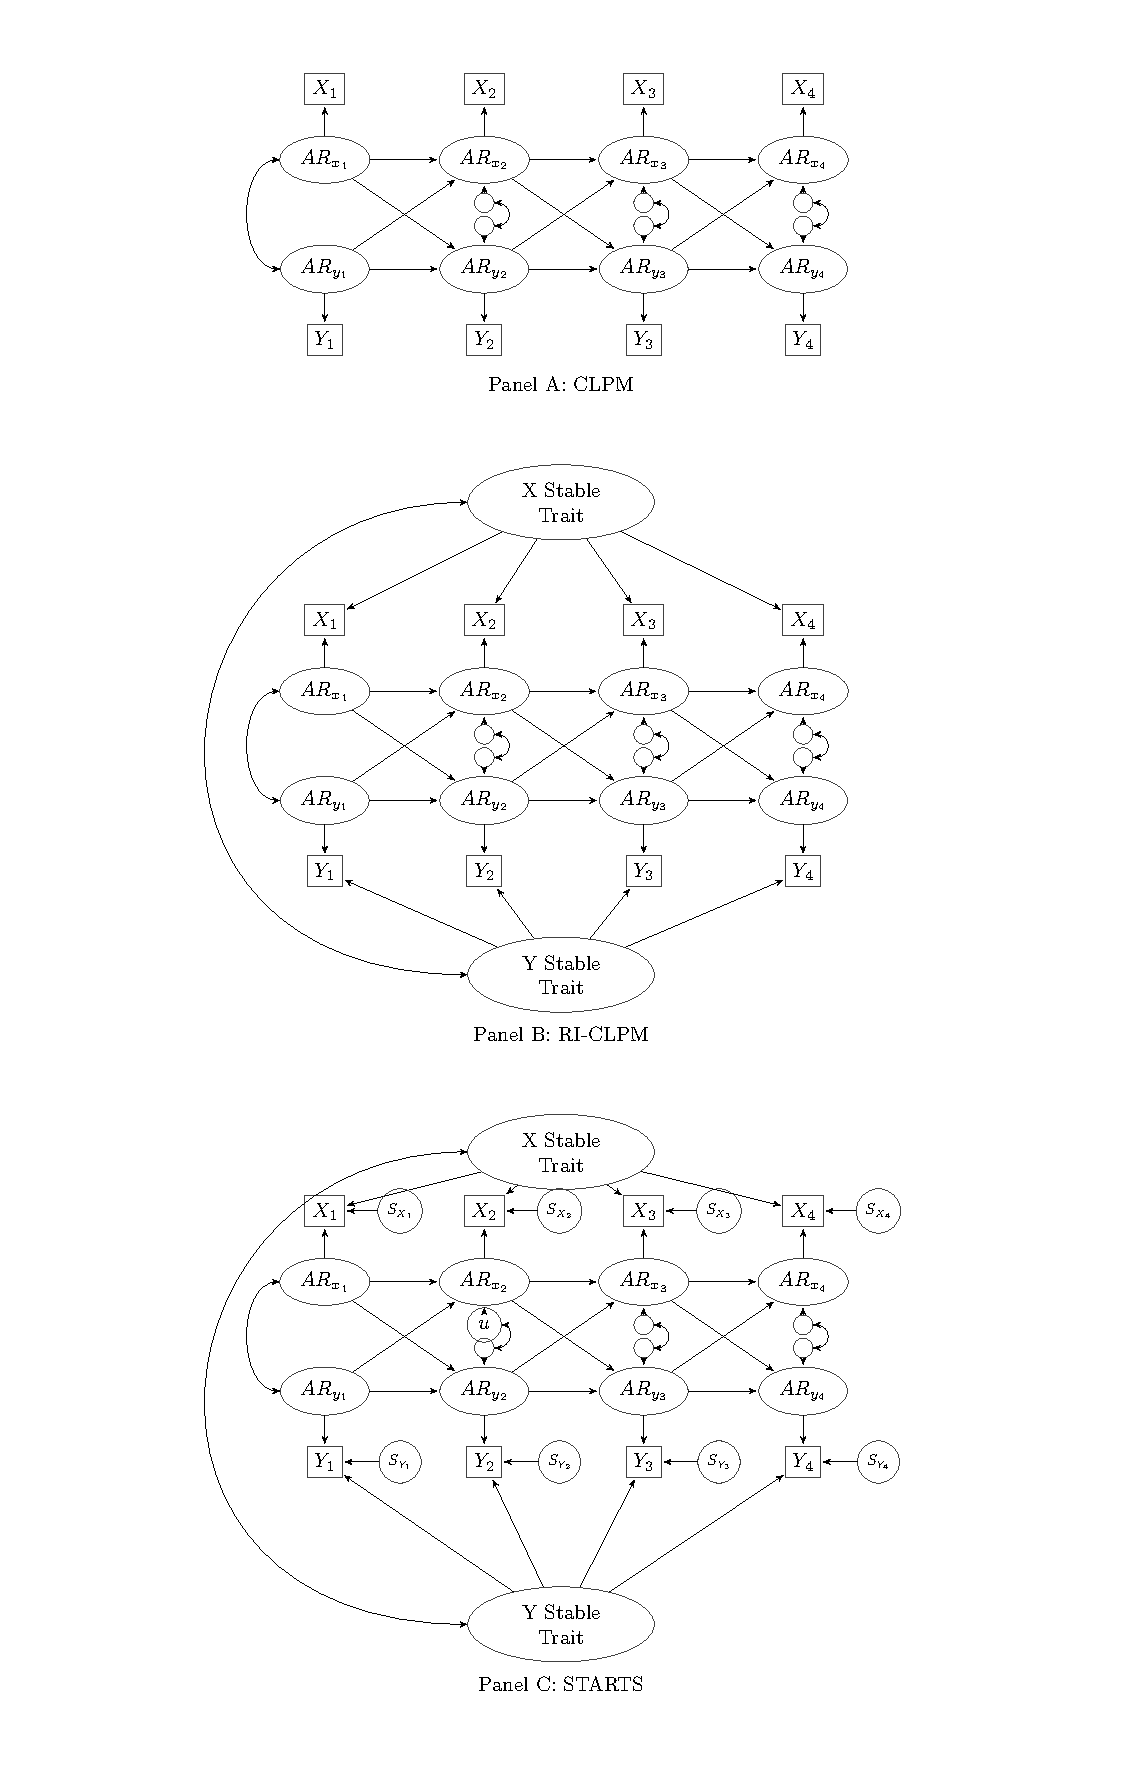
\includegraphics[height=0.9\textheight]{images/comboFigure} \caption{Diagram of the three models used in this paper.}\label{fig:riclpmFig}
\end{figure}

\hypertarget{the-ambiguous-nature-of-between-versus-within}{%
\subsection{The Ambiguous Nature of ``Between'' Versus ``Within''}\label{the-ambiguous-nature-of-between-versus-within}}

In presenting the RI-CLPM, Hamaker et al. (2015) emphasized that a strength was its ability to separate between-person effects from within-person effects. Critics of the RI-CLPM focus on this distinction when explaining their concerns with the model. The terms ``within-person'' and ``between-person,'' however, are ambiguous. As Usami (2021) recently noted, these terms are used differently in different contexts. I posit that this ambiguity and inconsistent usage has led to incorrect interpretations of the RI-CLPM and its alternatives.

When describing the RI-CLPM, Orth et al. (2021) argued that ``a potential disadvantage of the proposed alternatives to the CLPM is that they estimate within-person prospective effects only, but not between-person prospective effects'' (p.~1014). They go on to note that ``in many fields researchers are also interested in gaining information about the consequences of between-person differences'' (p.~1014). Similarly, in their critique of the RI-CLPM, Lüdtke and Robitzsch (2021) cautioned that ``researchers should be aware that within-person effects are based on person-mean centered (i.e., ipsatized) scores that only capture temporary fluctuations around individual person means'' which would be ``less appropriate for understanding the potential effects of causes that explain differences between persons'' (p.~18). Thus, these critics' central objection to the RI-CLPM is that it isolates within-person effects when sometimes that is not desirable\footnote{Though Lüdtke and Robitzsch (2021) did also articulate some additional concerns about the ability of the RI-CLPM to adequately account for unobserved confounders.}. But what is a within-person effect?

When answering this question, both Lüdtke and Robitzsch (2021) and Orth et al. (2021) are precise but inconsistent. For instance, Orth et al. (2021) initially state that ``in the RI-CLPM, a cross-lagged effect indicates whether a within-person deviation from the trait level of one construct has a prospective effect on change in the within-person deviation from the trait level of the other construct'' (p.~1014). This emphasis on ``deviations from the trait level'' reflects an accurate interpretation of the ``within-person'' part of the RI-CLPM. Similarly, Lüdtke and Robitzsch (2021) initially describe the within-person parts of the RI-CLPM as ``deviations from between-person parts'' of the model (p.~2), which is also correct. However, both authors later restate these description in ways that are either less precise or wrong. Importantly, the specific reasons both authors provide for preferring the CLPM to the RI-CLPM follow directly from the incorrect version of their description.

For instance, Orth et al. (2021) rephrase their original statement about ``deviations from the trait level'' to say that a within-person effect (in the context of their substantive example---a test of the causal effect of self-esteem on depression) means that ``When individuals have lower self-esteem than usual, they will experience a subsequent increase in depression.'' But what is this ``usual'' level from which people deviate? Can we interpret the random intercept from the RI-CLPM as a person's individual mean (as Lüdtke \& Robitzsch, 2021, did) or their ``usual level?'' And what exactly is left after scores are deviated from this random intercept?

Both Orth et al. (2021) appear to (incorrectly) assume that by including a random intercept, the RI-CLPM removes all between-person variance from the cross-lagged part of the model. For example, Orth et al. (2021) state this explicitly: They argue that ``a limitation of the RI-CLPM is that it does not provide any information about the consequences of between-person differences. In the RI-CLPM, the between-person differences are relegated to the random intercept factors'' (p.~1026). But this statement reflects a fundamental misunderstanding of the RI-CLPM, one that results from the ambiguous use of the terms ``between'' and ``within.'' Later on the same page, Orth et al.~state that ``The RI-CLPM includes {[}an{]} unrealistic assumption, specifically that the between-person variance in constructs is perfectly stable'' (p.~1026). But again, this is wrong: The authors who proposed the RI-CLPM simply restricted the term ``between-persons'' to refer the variance that is perfectly stable over time. This is an issue of terminology. The RI-CLPM does not assume that all between-persons variance is perfectly stable, it simply \emph{defines} ``between-persons'' variance as the variance that \emph{is} perfectly stable. There is clearly between-person variance (broadly defined) left in the cross-lagged part of the model.

\hypertarget{an-example}{%
\subsection{An Example}\label{an-example}}

To demonstrate, take the following example, where data are generated from a true autoregressive model with cross-lagged paths. In other words, the data-generating model looks like Panel A of Figure \ref{fig:riclpmFig}. For comparison with the substantive discussion by Orth et al., let's assume that the predictor is self-esteem and the outcome is depression. Specifically, in this example, I generated data for 10 waves of self-esteem and depression data, with no random intercept, starting variance of 1 for self-esteem and depression, stabilities of .5 for each, true cross-lagged paths of .50 from self-esteem to depression and .00 from depression to self-esteem. I also specified a Wave 1 correlation between self-esteem and depression of -.5. The code for the function to generate the data is available \href{https://github.com/rlucas11/starts/blob/main/gen_starts.R}{here} and included in the appendix.

According to Orth et al. (2021), significant cross-lagged paths from self-esteem to depression in this model can be interpreted to mean that ``When individuals have low self-esteem (relative to others), they will experience a subsequent rank-order increase in depression compared to individuals with high self-esteem.'' In other words, this model links between-person differences in self-esteem at Time 1 to between-person differences in depression at Time 2. They argue that this is precisely what many researchers would want to estimate in many common situations.

They also argue that when you test a model that includes random intercepts, the interpretation of the cross-lagged paths change. They state that a significant cross-lagged path in the context of the RI-CLPM means that ``When individuals have lower self-esteem than usual, they will experience a subsequent increase in depression'' (p.~1014) I think the problem is that what is captured by the ``stable trait'' in the RI-CLPM model is potentially (and frequently) different than a person's ``average level'' or ``usual level.'' I think that these two things can be very different, both conceptually and empirically. This is because the stable trait does not incorporate all between-person variance; it only includes variance that is perfectly stable across all waves. So what a substantial cross-lagged path really reflects in a RI-CLPM context is that ``When individuals have lower self-esteem \emph{than what would be predicted from their levels on the stable trait}, they will experience a subsequent increase in depression.''

This distinction may sound subtle, but it is important. For one thing, even when clear ``between-person'' differences exist in the data---for instance, in the data I generated---if one tries to fit the RI-CLPM to data without a stable-trait component, the estimate for the variance of the random intercept will be zero. If the RI-CLPM simply took what between-person variance exists and ``relegated'' it to a stable-trait component that reflected a person's long-term average, you would always be able to find a random intercept as long as some reasonably stable between-person variance exists.

Moreover, although one will not always find random-intercept variance when testing the RI-CLPM on data with real between-person differences, it is always possible to do what Orth et al. (2021) and Lüdtke and Robitzsch (2021) claim the RI-CLPM does, which is to ipsatize the predictor and outcome variables by deviating them from a person's mean and then computing cross-lagged associations using this mean-deviated data. This procedure truly does separate all between-person variance from within; there would be no variance left in person-level means after ipsatizing in this way. To demonstrate and compare ipsatizing to fitting an RI-CLPM model, I subtracted each person's mean self-esteem score and mean depression score in each wave and then reran the CLPM using these ipsatized data. For comparison, I also ran the RI-CLPM on the original, undeviated data\footnote{Note that the CLPM model will often result in nonpositive-definite matrices with the mean-deviated data. I chose a random seed that generates data where all models converge, but this may not be true for other randomly generated data. In addition, as expected, fitting the RI-CLPM to data with a true autoregressive structure resulted in negative variances (because the true variance of the random-intercept is zero, so estimates can drop below). The estimates for the RI-CLPM model in the table come from a solution with negative variances and are provided simply to show that they are close to the true parameters, even when the overall model solution is inadmissable.}. The first three pairs of columns from Table \ref{tab:meanDeviatedTable} show the relevant estimates for the original CLPM and these two alternatives.

\begin{lltable}

\begin{TableNotes}[para]
\normalsize{\textit{Note.} The estimates for the CLPM columns reflect the CLPM fit to the original data. The estimates in the Deviated ClPM columns reflect the CLPM fit to the mean-deviated data. The estimates for the RI-CLPM column reflect the RI-CLPM fit to the original data. The estimates for the RI-CLPM column reflect the RI-CLPM fit to the original data with the stable trait variance added.}
\end{TableNotes}

\begin{longtable}{lrrrrrrrr}\noalign{\getlongtablewidth\global\LTcapwidth=\longtablewidth}
\caption{\label{tab:meanDeviatedTable}Comparison of Estimates for Cross-Lagged Effects}\\
\toprule
 & \multicolumn{2}{c}{CLPM} & \multicolumn{2}{c}{Deviated CLPM} & \multicolumn{2}{c}{RI-CLPM} & \multicolumn{2}{c}{RI-CLPM with Trait} \\
\cmidrule(r){2-3} \cmidrule(r){4-5} \cmidrule(r){6-7} \cmidrule(r){8-9}
 & \multicolumn{1}{c}{est} & \multicolumn{1}{c}{se} & \multicolumn{1}{c}{est} & \multicolumn{1}{c}{se} & \multicolumn{1}{c}{est} & \multicolumn{1}{c}{se} & \multicolumn{1}{c}{est} & \multicolumn{1}{c}{se}\\
\midrule
\endfirsthead
\caption*{\normalfont{Table \ref{tab:meanDeviatedTable} continued}}\\
\toprule
 & \multicolumn{2}{c}{CLPM} & \multicolumn{2}{c}{Deviated CLPM} & \multicolumn{2}{c}{RI-CLPM} & \multicolumn{2}{c}{RI-CLPM with Trait} \\
\cmidrule(r){2-3} \cmidrule(r){4-5} \cmidrule(r){6-7} \cmidrule(r){8-9}
 & \multicolumn{1}{c}{est} & \multicolumn{1}{c}{se} & \multicolumn{1}{c}{est} & \multicolumn{1}{c}{se} & \multicolumn{1}{c}{est} & \multicolumn{1}{c}{se} & \multicolumn{1}{c}{est} & \multicolumn{1}{c}{se}\\
\midrule
\endhead
Stability of Self-Esteem & 0.50 & 0.00 & 0.36 & 0.00 & 0.50 & 0.00 & 0.50 & 0.00\\
Stability of Depression & 0.50 & 0.00 & 0.38 & 0.00 & 0.50 & 0.00 & 0.50 & 0.00\\
Self-Esteem Predicted by Depression & 0.00 & 0.00 & 0.17 & 0.00 & 0.00 & 0.00 & 0.00 & 0.00\\
Depression Predicted by Self-Esteem & -0.50 & 0.00 & -0.49 & 0.00 & -0.50 & 0.00 & -0.50 & 0.00\\
Variance of Self-Esteem AR Trait & 1.01 & 0.01 & 0.87 & 0.01 & 1.01 & 0.02 & 1.02 & 0.02\\
Variance of Depression AR Trait & 0.99 & 0.01 & 0.79 & 0.01 & 0.99 & 0.02 & 0.99 & 0.02\\
Covariance Between AR Components & -0.49 & 0.01 & -0.37 & 0.01 & -0.49 & 0.01 & -0.50 & 0.01\\
Variance of Self-Esteem Stable Trait &  &  &  &  & 0.00 & 0.00 & 0.49 & 0.01\\
Variance of Depression Stable Trait &  &  &  &  & 0.00 & 0.01 & 0.51 & 0.01\\
Covariance of Stable Traits &  &  &  &  & 0.00 & 0.01 & -0.40 & 0.01\\
\bottomrule
\addlinespace
\insertTableNotes
\end{longtable}

\end{lltable}

As can be seen in this table, the estimates from the mean-deviated CLPM model are quite different both from the CLPM and the RI-CLPM fit to the original (undeviated) data. In contrast, the estimates from the RI-CLPM are almost identical to those from the CLPM. Thus, the RI-CLPM is not equivalent to a CLPM with ipsatized (mean-deviated) data. Again, the cross-lagged part of the RI-CLPM reflects deviations from the latent stable trait, and if there is no variance in this stable trait, then the RI-CLPM is equivalent to the CLPM. The fact that the CLPM is a reduced version of the RI-CLPM where the random-intercept variance is set to 0 is, of course, obvious just by looking at the models. The point of this example is to clarify what that means for the interpretation of these cross-lagged paths.

A potential response to this example would be to acknowledge that using the RI-CLPM will not artificially create random-intercept variance when it does not exist, while still arguing that when stable between-person variance does exist, the model somehow distorts the cross-lagged paths. But this is also not correct. Imagine that we take the same data from above, but now we add some stable-trait variance. Let's assume for this example that the added stable-trait variance is just shared method variance. Specifically, we can generate data representing a method factor for self-esteem and one for depression. In generating these data, I set the variance of these stable-trait components to .50, and I assumed that the stable traits are pretty strongly (and negatively, given the direction of the items) correlated (though this doesn't really matter for this specific example). We can then just add the generated method-variance scores to the original data.

If we fit the RI-CLPM to the combined data, you get exactly what you'd expect: The estimates for the random intercept simply reflect the method variance we've added. These results are shown in the final columns of Table \ref{tab:meanDeviatedTable}. The variance of each estimated random intercept is about .50 and the covariance is about -.40 (for a correlation of -.80). These random intercepts don't capture any of the between-person differences in the original data (which are substantial) because the original individual differences are not \emph{perfectly} stable across waves. In other words, the model does not, as Orth et al.~suggested ``relegate all between-person differences to the random intercept,'' it simply pulls out those between-person differences that are completely stable over time.

More importantly, Table \ref{tab:meanDeviatedTable} shows that the estimates for the original autoregressive, cross-lagged part of the model are the same as what you get when you run the CLPM on the original data. The variances, stabilities, and cross-lagged paths are the same (as they should be). Contrary to Orth et al., the cross-lagged part of the model still links the same between-person variance in self-esteem at Time 1 to between-person variance in depression at Time 2. The interpretation of this part of the model is exactly the same when no stable-trait variance exists as it is when there is stable-trait variance, but that stable-trait variance is modeled using the RI-CLPM. Specifically, in the RI-CLPM, the cross-lagged effects still assess whether those who have high self-esteem relative to others at Time 1 report larger changes in depression over time. The difference is that these effects have now been adjusted for stable differences in measurement error; they have certainly not been ``ipsatized'' in any way.

Of course, in real data, we typically do not know whether the stable-trait variance that exists reflects something that is clearly not theoretically interesting (as is true of method variance). My point is that adding some stable trait variance (in this case, method variance) and then modeling this stable variance using the RI-CLPM doesn't suddenly make the cross-lagged part any more ``within-persons'' than it was before. Indeed, I am pretty sure that what Orth et al. (2021) would call a between-persons model---the CLPM fit to the original data I generated---would actually be described by Hamaker et al. (2015) as a within-persons model, not because of what the model is doing, but simply because there is no stable-trait variance. Again, this is an issue of terminology.

An additional response that the critics of the RI-CLPM could make is that there is some important reason to avoid separating purely stable between-person variance from the between-person variance that remains in the autoregressive part of an RI-CPLM or STARTS model when testing causal associations with longitudinal data. However, this is \emph{not} the argument that these critics made. They explicitly state that their objection to the RI-CLPM was that it removed all between person differences from the autoregressive/cross-lagged part of the model, which resulted in cross-lagged paths that capture only associations between ipsatized scores (which reflect deviations from people's usual level) for the predictor and outcome. Perhaps there is a reason why both types of individual differences (those captured by the stable trait and those that remain in the autoregressive part of the model) would be expected to be associated with wave-to-wave changes, but these reasons were not put forth.

It is noteworthy that neither Lüdtke and Robitzsch (2021) nor Orth et al. (2021) described a data-generating model that would result in biased estimates or incorrect conclusions if analyzed incorrectly using the RI-CLPM. As I demonstrated above, generating data from the model that they claim to prefer---the CLPM---results in correct estimates (despite inadmissable solutions due to negative estimated variances) when analyzed using the RI-CLPM. I believe that it is not possible to specify a data-generating model that corresponds to the processes that the critics describe that would also lead to incorrect estimates when analyzed using the RI-CLPM\footnote{Lüdtke and Robitzsch (2021) did show that the RI-CLPM cannot successfully control for all types of confounds, but this is an issue that is distinct from the question of whether we can simply recover the structure of these variables over time. Of course, it is possible to specify data-generating models that do result in data that, when analyzed using the RI-CLPM, lead to incorrect conclusions (including the more complex models described by Usami et al. (2019)). My point is that the critics of the RI-CLPM have not provided a model that matches the processes that they describe and also results in incorrect estimates when modeled using the RI-CLPM.}.

\hypertarget{the-source-of-confusion}{%
\subsection{The Source of Confusion}\label{the-source-of-confusion}}

I think the source of the confusion about the RI-CLPM is that people use the terms ``between'' and ``within'' in different ways in different contexts (Usami, 2021). Many people (at least in my field) are used to thinking of the differences between within-person effects and between-person effects in the context of multilevel modeling. We are often warned that when testing multilevel models, if we are not careful about how we enter variables into the model, what may look like within-person effects (e.g., the ``Level-1'' effects in repeated-measures data analyzed in a multilevel modeling framework) can actually reflect a mix of between- and within-person associations. The recommended solution is often to person-center the predictor (e.g., Enders \& Tofighi, 2007), where each observation now reflects a deviation from a person's mean. When centering this way, the Level-1 part of these models completely separates within-person variance from between---all between-person variance has been removed from this part of the model (at least in the predictor).

So when methodologists talk about separating ``within'' from ``between,'' there are at least two possible meanings to this distinction. In the first (used by Curran et al., 2014; Hamaker et al., 2015, and others to describe models with a stable-trait component), ``between-person'' variance and effects refer to those that are perfectly stable over time, and ``within-person'' variance and effects include everything that is not perfectly stable. In the second meaning, ``within-person'' variance and effects are those that involve ipsatized scores from which all ``between-person'' variance (broadly defined) has been removed. These two meanings are not equivalent.

Why does this matter? Critics of the RI-CLPM appear to interpret the within/between distinction in the ``ipsatizing'' way, and they derive their concerns about the model from this interpretation. They explicitly state that their primary reason for avoiding the RI-CLPM is that it focuses so narrowly on within-person deviations from a person's ``usual level''. For instance, as previously noted, Lüdtke and Robitzsch (2021) cautioned that ``researchers should be aware that within-person effects are based on person-mean centered (i.e., ipsatized) scores that only capture temporary fluctuations around individual person means'' which would be ``less appropriate for understanding the potential effects of causes that explain differences between persons.'' But if the first part of that statement is incorrect, then the second would not follow. Similarly, all of the limitations of the RI-CLPM and all of the reasons for preferring the CLPM to the RI-CLPM discussed by Orth et al. (2021, p. 1026) are based on an incorrect description of what the cross-lagged part of the RI-CLPM really does. Orth et al.~conclude that ``the RI-CLPM does not allow testing what many researchers \ldots{} are interested in: the prospective between-person effect'' (p.~1026). I think the very term ``prospective between-person effect'' reflects the confusion about the meaning of the terms ``between'' and ``within'' that I noted; but to the extent that such a thing exists, the RI-CLPM captures it just as well as the CLPM.

\hypertarget{beyond-within-and-between}{%
\section{Beyond ``Within'' and ``Between''}\label{beyond-within-and-between}}

Given the ambiguity of the terms ``within'' and ``between'' in the context of models like the CLPM and its alternatives, it can be helpful discuss benefits of the RI-CLPM over the CLPM without referring to this distinction\footnote{Ultimately, I think that Hamaker et al.'s (2015) framing is a more precise way of saying the same thing; my point is that we don't necessarily need to the within/between framing to understand the problems with the CLPM.}. Specifically, the RI-CLPM is useful because it tests an extremely plausible alternative explanation of the underlying pattern of correlations that is being modeled when the CLPM is used.

The logic of the CLPM is very similar to the logic of any other regression model where we assess whether one variable predicts another after controlling for relevant confounds. When we test whether Time 1 X predicts Time 2 Y after controlling for Time 1 Y, we hope to capture whether there is something unique about X---something that cannot be explained by the concurrent association between X and Y---that helps us predict Y at a later time. But as Westfall and Yarkoni (2016) pointed out, if the measure that we include as a control (i.e., Time 1 X) is not a perfect measure of what we're trying to account for, then it is possible---indeed, quite easy---to find spurious ``incremental validity'' effects. This, I think, is a simpler way of thinking about the strengths of the RI-CLPM relative to the CLPM.

\hypertarget{its-incredibly-easy-to-find-spurious-cross-lagged-effects}{%
\subsection{It's Incredibly Easy to Find Spurious Cross-Lagged Effects}\label{its-incredibly-easy-to-find-spurious-cross-lagged-effects}}

The problem with the CLPM is that is easy---in fact, incredibly easy---to find spurious cross-lagged associations under conditions that are extremely likely in the typical situations where the CLPM is used. Hamaker et al.~(2015) conducted simulations to show that the estimates from a cross-lagged panel model were often biased in realistic situations. I don't think they went far enough, though, in describing the practical implications of these simulations or showing just how likely spurious effects are in realistic situations. So the rest of this paper simply builds on their simulations and tries to clarify when such spurious effects are likely to occur.

\hypertarget{the-simulations}{%
\subsubsection{The Simulations}\label{the-simulations}}

When considering what types of situations to simulate, I focus on realistic scenarios for the types of data to which the CLPM is likely to be applied. For instance, it is likely that most variables that psychologists choose to study over time have a STARTS-like structure, where stability declines with increasing interval length (reflecting an autoregressive structure), yet this decline approaches or reaches an asymptote where further increases in interval length are no longer associated with declines in stability (reflecting the influence of a stable trait). It is also likely that most measures of psychological constructs have some amount of pure state variability, which could reflect measurement error and true state-like influences. Starting with this assumption, it is then possible to test how variation in these factors affect the estimated cross-lagged paths when the CLPM is used.

Because the focus of this paper is on examining the effects of unmodeled stable trait variance, I set the variance of the stable trait component for the predictor and outcome to be 1 in all simulations. I then varied the ratio of autoregressive variance to stable-trait variance across four levels: 0, .5, 1, and 2. Similarly, I varied the ``reliability'' of the measures (defining reliability as the proportion of variance due to stable-trait and autoregressive-trait variance) across three levels: .5, .7, and .9. Even the lowest level is not unrealistic, given that the state component includes both measurement error and reliable state variance. Finally, I varied the size of the correlation between the stable traits across four levels: .1, .3, .5, and .7. I ran 1,000 simulations for each of six sample sizes: 25, 50, 100, 250, 500, and 1,000). In all simulations, I set the correlation between the initial autoregressive variance components for the predictor and outcome to be .50 and the stability of the autoregressive components to be .50 (though, later, I discuss some modifications to this). I also set the correlations between state components to be 0. Consistent with the canonical STARTS model, I included a stationarity constraint, so that variances, correlations, and stability coefficients are constrained to be equal over time.

After generating the data, I tested a simple two-wave CLPM, keeping track of the average size of the estimated cross-lagged paths and the number of cross-lagged paths that were significant at a level of .05. Note that researchers are often interested in determining which of the two variables in the model has a causal impact on the other rather than on simply testing the effect of one predictor on an outcome. Thus, an effect of X on Y, Y on X, or both would often be interpreted as a ``hit'' in common applications of the CLPM. This means that error rates are typically elevated in the CLPM even without unmodeled stable-trait effects unless corrections for multiple comparisons are used. In these simulations, I report the percentage of runs that result in at least one significant cross-lagged effect (out of two tested), and readers can interpret these results either in comparison to a baseline error rate of 5\% or 10\% depending on how these multiple comparisons are considered.

Finally, although I focus on the common two-wave CLPM design, it is important to note that more waves of data lead to increased power to detect smaller effects---even spurious effects. This means that spurious cross-lagged associations are more likely to be found with better, multi-wave designs. Thus, I will also present results from simulations with more waves of data after presenting the primary results.

\begin{figure}
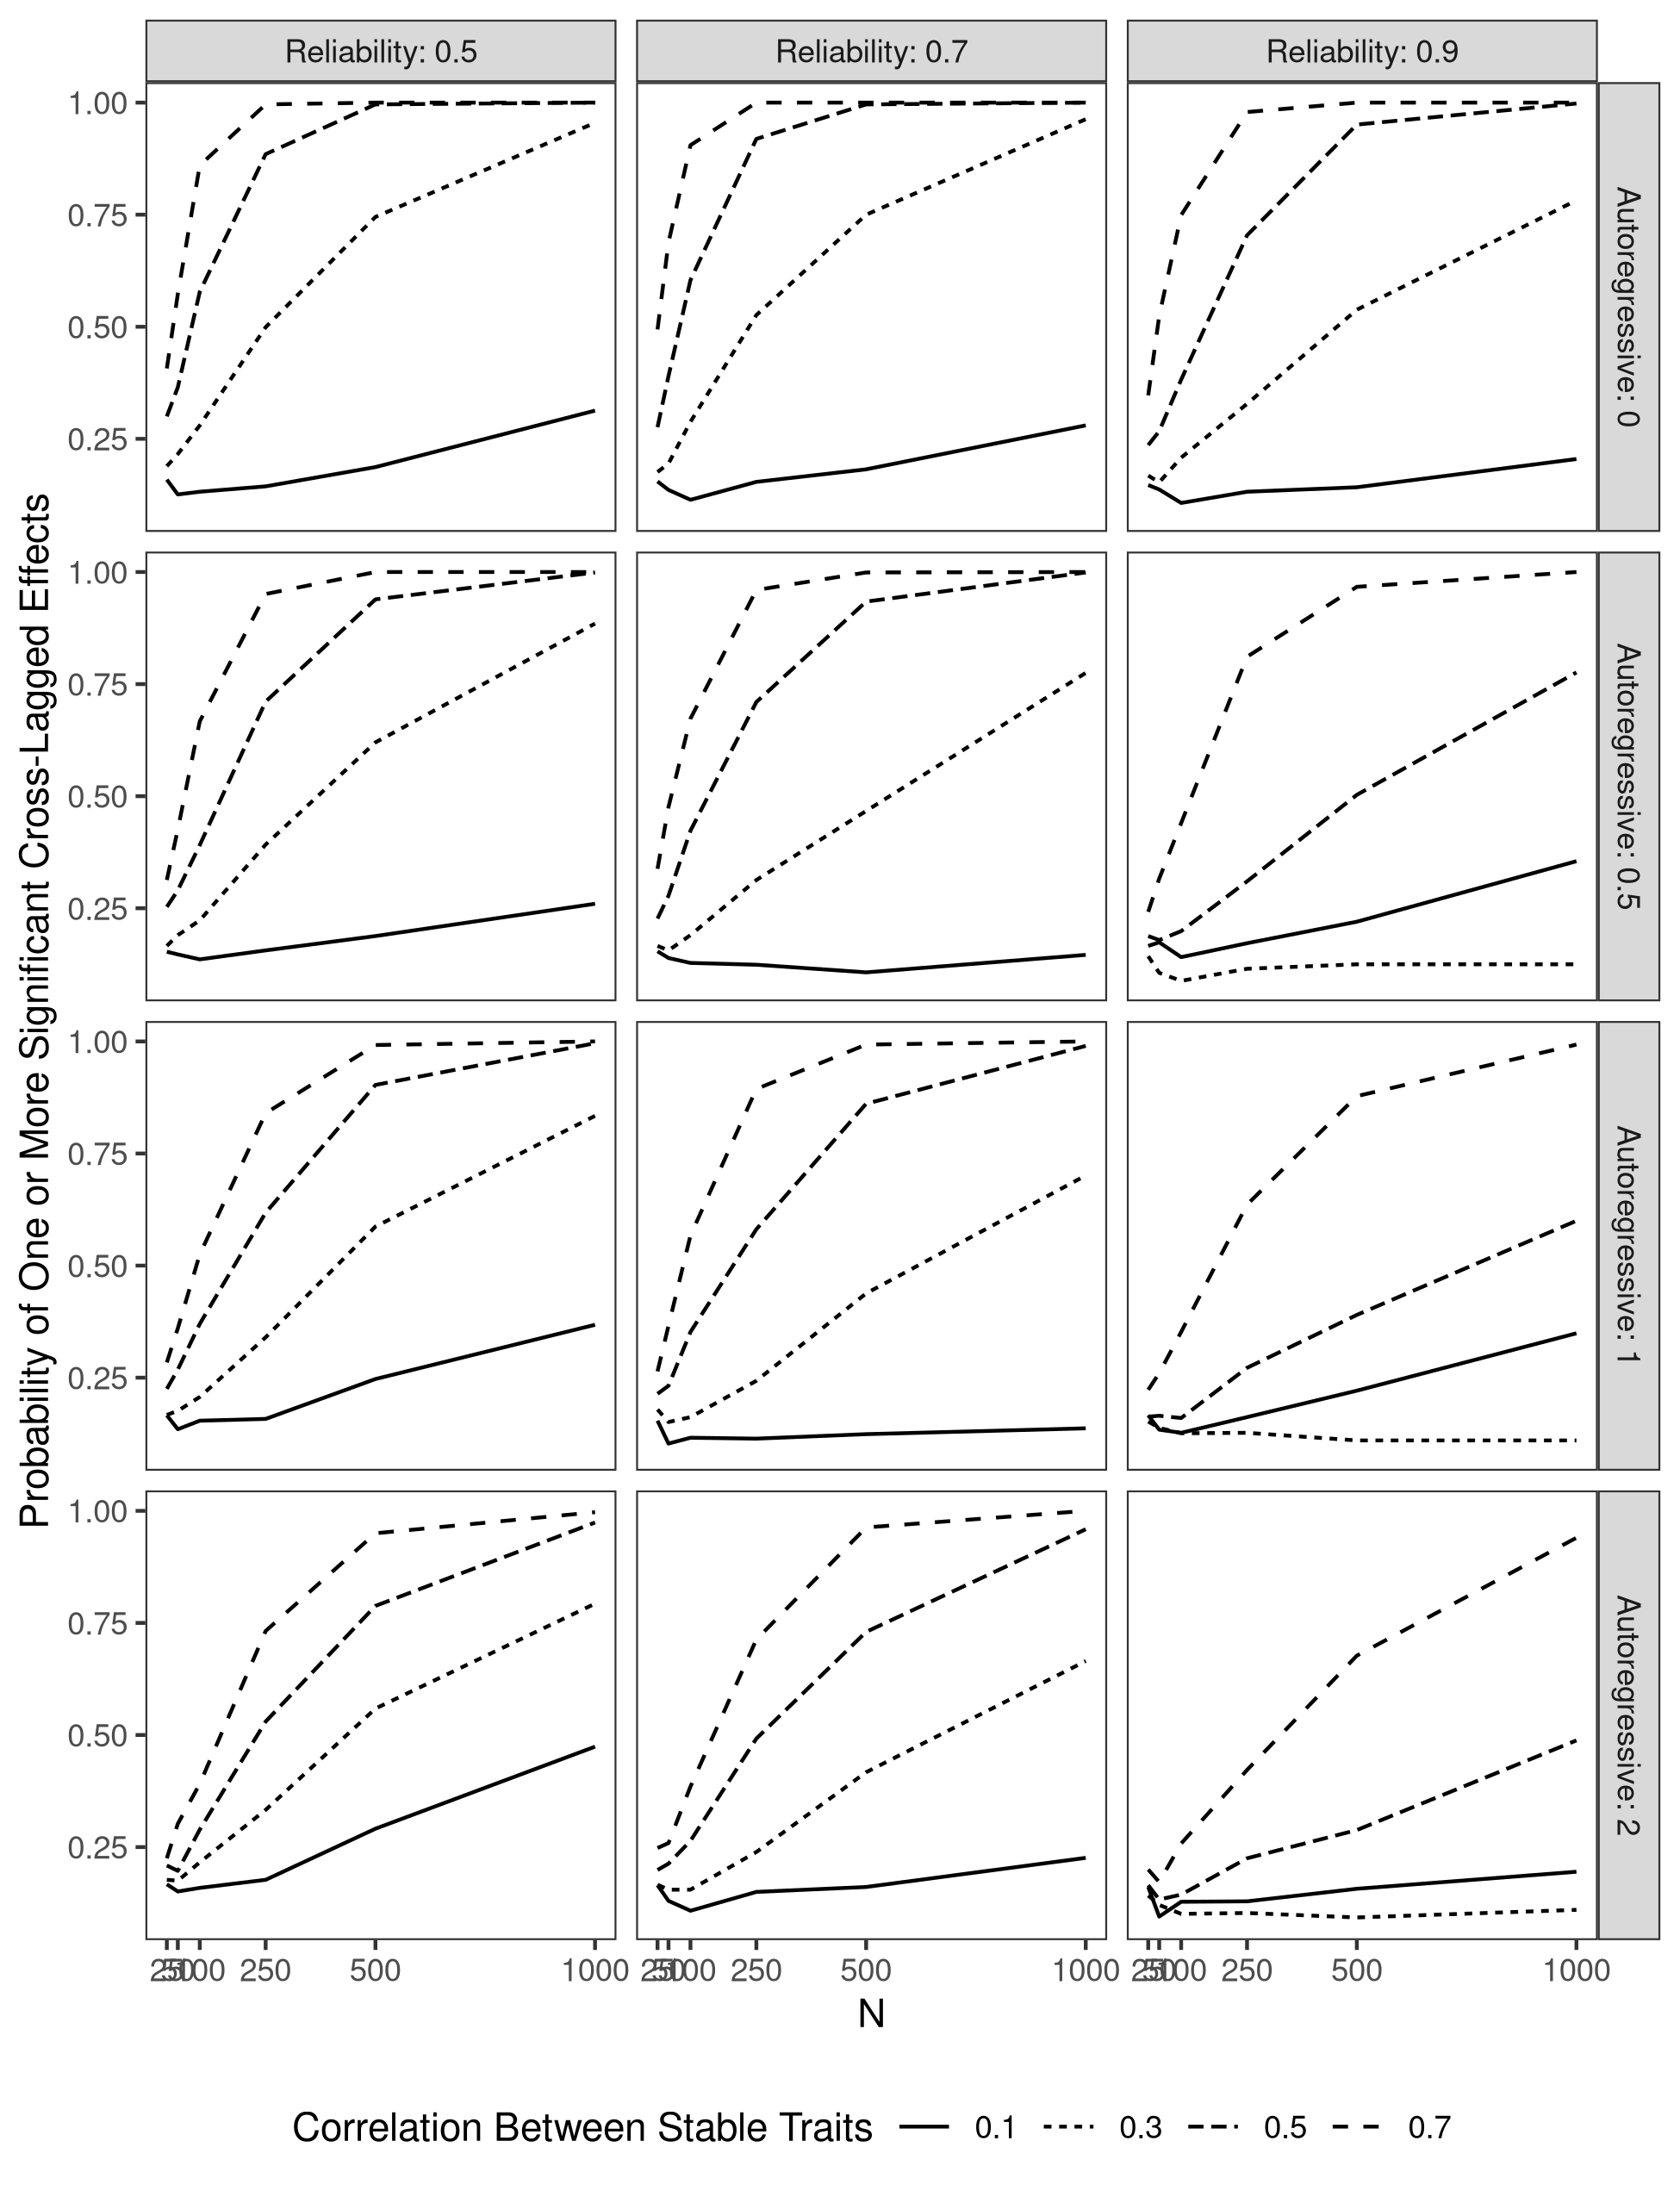
\includegraphics[width=6.5in,height=0.9\textheight]{images/2WaveSimulation} \caption{Simulation results for two-wave CLPM. Columns reflect different reliabilities. Rows reflect different ratios of autoregressive to stabler-trait variance. Lines reflect different correlations between stable-trait components.}\label{fig:simFig}
\end{figure}

\begin{table}[tbp]

\begin{center}
\begin{threeparttable}

\caption{\label{tab:simTab}Average Estimated Cross-Lagged Paths In Each Simulation Condition}

\begin{tabular}{rrrrr}
\toprule
 &  & \multicolumn{3}{c}{Reliability} \\
\cmidrule(r){3-5}
Stable Trait r & \multicolumn{1}{c}{AR Variance Ratio} & \multicolumn{1}{c}{0.5} & \multicolumn{1}{c}{0.7} & \multicolumn{1}{c}{0.9}\\
\midrule
0.10 & 0\% & 0.03 & 0.02 & 0.01\\
 & 50\% & 0.03 & 0.01 & -0.02\\
 & 100\% & 0.03 & 0.01 & -0.03\\
 & 200\% & 0.04 & 0.02 & -0.02\\ \midrule
0.30 & 0\% & 0.08 & 0.06 & 0.03\\
 & 50\% & 0.07 & 0.05 & 0.01\\
 & 100\% & 0.07 & 0.05 & 0.01\\
 & 200\% & 0.07 & 0.05 & 0.01\\ \midrule
0.50 & 0\% & 0.13 & 0.12 & 0.06\\
 & 50\% & 0.11 & 0.10 & 0.05\\
 & 100\% & 0.10 & 0.09 & 0.04\\
 & 200\% & 0.09 & 0.08 & 0.04\\ \midrule
0.70 & 0\% & 0.20 & 0.20 & 0.11\\
 & 50\% & 0.16 & 0.16 & 0.10\\
 & 100\% & 0.14 & 0.14 & 0.09\\
 & 200\% & 0.12 & 0.11 & 0.07\\
\bottomrule
\end{tabular}

\end{threeparttable}
\end{center}

\end{table}

The proportion of simulations that resulted in at least one significant cross-lagged effect are presented in Figure \ref{fig:simFig}. The X-axis shows results for different sample sizes. The Y-axis reflects the percentage of runs in which a significant (spurious) cross-lagged path was found. Ideally, this would be close to 10\% {[}FIX THIS, NOT EXACTLY 10\%{]}, which would be the error rate without taking multiple comparisons into account. The columns reflect variation in the reliability of the measures. The rows reflect variation in the ratio of autoregressive variance to stable-trait variance. The individual lines in each plot reflect different correlations between the two stable traits. The averaged estimates for the cross-lagged paths in each set of simulations (averaging across sample sizes, as this will not affect the estimated effect) is reported in Table \ref{tab:simTab}. So, when can you find spurious effect? Here are a few common situations.

\hypertarget{when-constructs-have-some-stable-trait-structure}{%
\subsubsection{When Constructs Have Some Stable-Trait Structure}\label{when-constructs-have-some-stable-trait-structure}}

If the measures include some amount of stable-trait variance--even if the stable traits are uncorrelated---it is likely that spurious cross-lagged paths will emerge. To be clear, this is most problematic when the correlations between the stable-trait components are quite high. However, error rates are elevated across most simulations. For instance, for the moment, ignore the effect of measurement error/state variance, and consider results in the third column of Figure \ref{fig:simFig}, where the reliability is a very high .9. Specifically, focus on the fourth row, where the ratio of autoregressive variance to stable-trait variance is 2:1. This panel reflects the least problematic set of values tested, and even here, error rates approach 100\% when correlations between the stable traits are strong (\emph{r} = .70) and sample sizes are large (\emph{N} = 1,000). Even when correlations are more moderate (e.g., \emph{r} = .5), however, these error rates approach 50\% in large samples.

Interestingly, error rates are not monotonically associated with the size of the correlation when reliability is high. Consider the panels in Rows 2, 3, and 4 of Column 3. In these panels, where the ratio of autoregressive variance to stable-trait variance is .5 or higher, the error rates for the lowest correlation tested (\emph{r} = .1, shown in the solid line) are actually higher than error rates for a higher stable-trait correlation of .3. A look at the actual estimates across simulations in Table \ref{tab:simTab} provides insight into why this is. This table shows that the average estimated cross-lagged path is actually negative when reliability is high, the correlation between the stable traits is low, and there is substantial amounts of autoregressive variance. These negative estimates emerge even though all associations among the latent components were specified to be positive. This effect can be demonstrated even more clearly by simulating data with a correlation between stable traits of zero, an equal amount of autoregressive and stable-trait variance, and no stable-trait variance whatsoever. In this case, the estimated cross-lagged paths will be approximately -.07. This is due to the fact that by ignoring the stable trait, the model overestimates the stability of X and Y, which means that the observed correlation between X at Time 1 and Y at Time 2 is lower than what would be expected based on the initial correlation between X and Y at Time 1 and the stability over time\footnote{This can be understood by using tracing rules. If we randomly generate data for 10,000 participants from the data-generating model just described, the correlation between \emph{X1} and \emph{X2} and between \emph{Y1} and \emph{Y2} are both around .75. The correlation between \emph{X1} and \emph{Y1} would be about .25, and the correlation between \emph{X1} and \emph{Y2} would be about .12. Fitting a CLPM to these data results in estimated stabilities for X and Y of approximately .77, and a correlation between \emph{X1} and \emph{Y1} of .25. These values would imply an observed correlation of \(.77 * .25 = .19\), which is greater than the actual correlation of .12. This results in the negative estimates for the cross-lagged paths.}. These simulations show that when the variables being examined have a trait-like structure, this can lead to spurious cross-lagged effects, even when the stable trait variance is not correlated. When correlations at the stable-trait level are strong, however, the effects of ignoring the stable-trait structure can be pronounced. In some realistic scenarios (e.g., moderate correlations between stable traits, reliabilities of .70, and sample sizes over 100), significant spurious correlations are almost guaranteed.

\hypertarget{when-measures-have-error-or-reliable-occasion-specific-variance}{%
\subsubsection{When Measures Have Error or Reliable Occasion-Specific Variance}\label{when-measures-have-error-or-reliable-occasion-specific-variance}}

The simulations described above focus on situations where reliability is very high. When there is measurement error or reliable state variance (as is very likely), this effect gets worse---potentially \emph{much} worse. Consider the panel in the first row and the first column of Figure \ref{fig:simFig}. In this case, reliability is set to .5 and there is no autoregressive variance. Error rates are very high, approaching 100\% with large samples, even when the stable-trait correlation is just .3. Even samples of 100 can result in spurious cross-lagged effects approximately 60\% of the time when stable traits are correlated .5.

This outcome is actually quite easy to understand. Indeed, we don't really need simulations at all to predict it. This result is a simple consequence of the issues that Westfall and Yarkoni (2016) discussed. Because X and Y are measured with error at each occasion, controlling for Time 1 Y when predicting Time 2 Y from Time 1 X does not fully account for the true association between X and Y. There will still be a residual association between Time 1 X and Time 2 Y, which can be accounted for by the freed cross-lagged path in the CLPM. The RI-CLPM (and the STARTS) are useful because they do a better job accounting for this underlying association than the CLPM.

One might argue that a model that just includes stable-trait variance and error (which is true of all simulations in the first row of Figure \ref{fig:simFig}) is unrealistic, as there is sure to be some form of autoregressive structure to most variables we study. That is true, but as the other rows of the figure show, the existence of this stable trait causes problems for the CLPM even when all three sources of variability (stable trait, autoregressive trait, and state) exist.

At this point, it's important to highlight the fact that at least some of these effects are due more to the existence of measurement error (or reliable state variance) than to the existence of the stable trait. For instance, we could simulate data with an autoregressive structure, set the variance of the stable trait components to be 0, and specify no cross-lagged paths, and even with high reliability, there will be enough power to detect spurious cross-lagged effects with just a couple hundred participants. Again, Westfall and Yarkoni's (2016) explanation can account for these results.

In addition, measurement error also affects estimates from the RI-CLPM. If we specify a data-generating model that includes all three sources of variance (stable trait, autoregressive trait, and state/measurement error), but no cross-lagged paths, the CLPM will find substantial cross-lagged effects, but so will the RI-CLPM (at least if the autoregressive components of X and Y are correlated). The reasons for this are the same as those discussed above. Note, this limitation of the RI-CLPM is not an argument \emph{for} the CLPM (though it is an argument for using the STARTS, when possible).

One response to the above simulations is to suggest that we simply need to use very reliable measures or perhaps model latent variables at each occasion instead of relying on observed variables with less than perfect reliability. This will certainly help, but it is important to remember that the ``state'' component in the STARTS model includes measurement error \emph{and} reliable occasion-specific variance. And reliable state variance will affect these results in exactly the same way as random measurement error. Unfortunately, we don't know how common this reliable state component is in real data, though we have at least some evidence that it can exist and be large enough to be meaningful (Lucas \& Donnellan, 2012). Thus, even the use of latent occasions in the CLPM can't solve this problem.

\hypertarget{when-there-are-many-assessment-waves}{%
\subsubsection{When There Are Many Assessment Waves}\label{when-there-are-many-assessment-waves}}

\begin{figure}
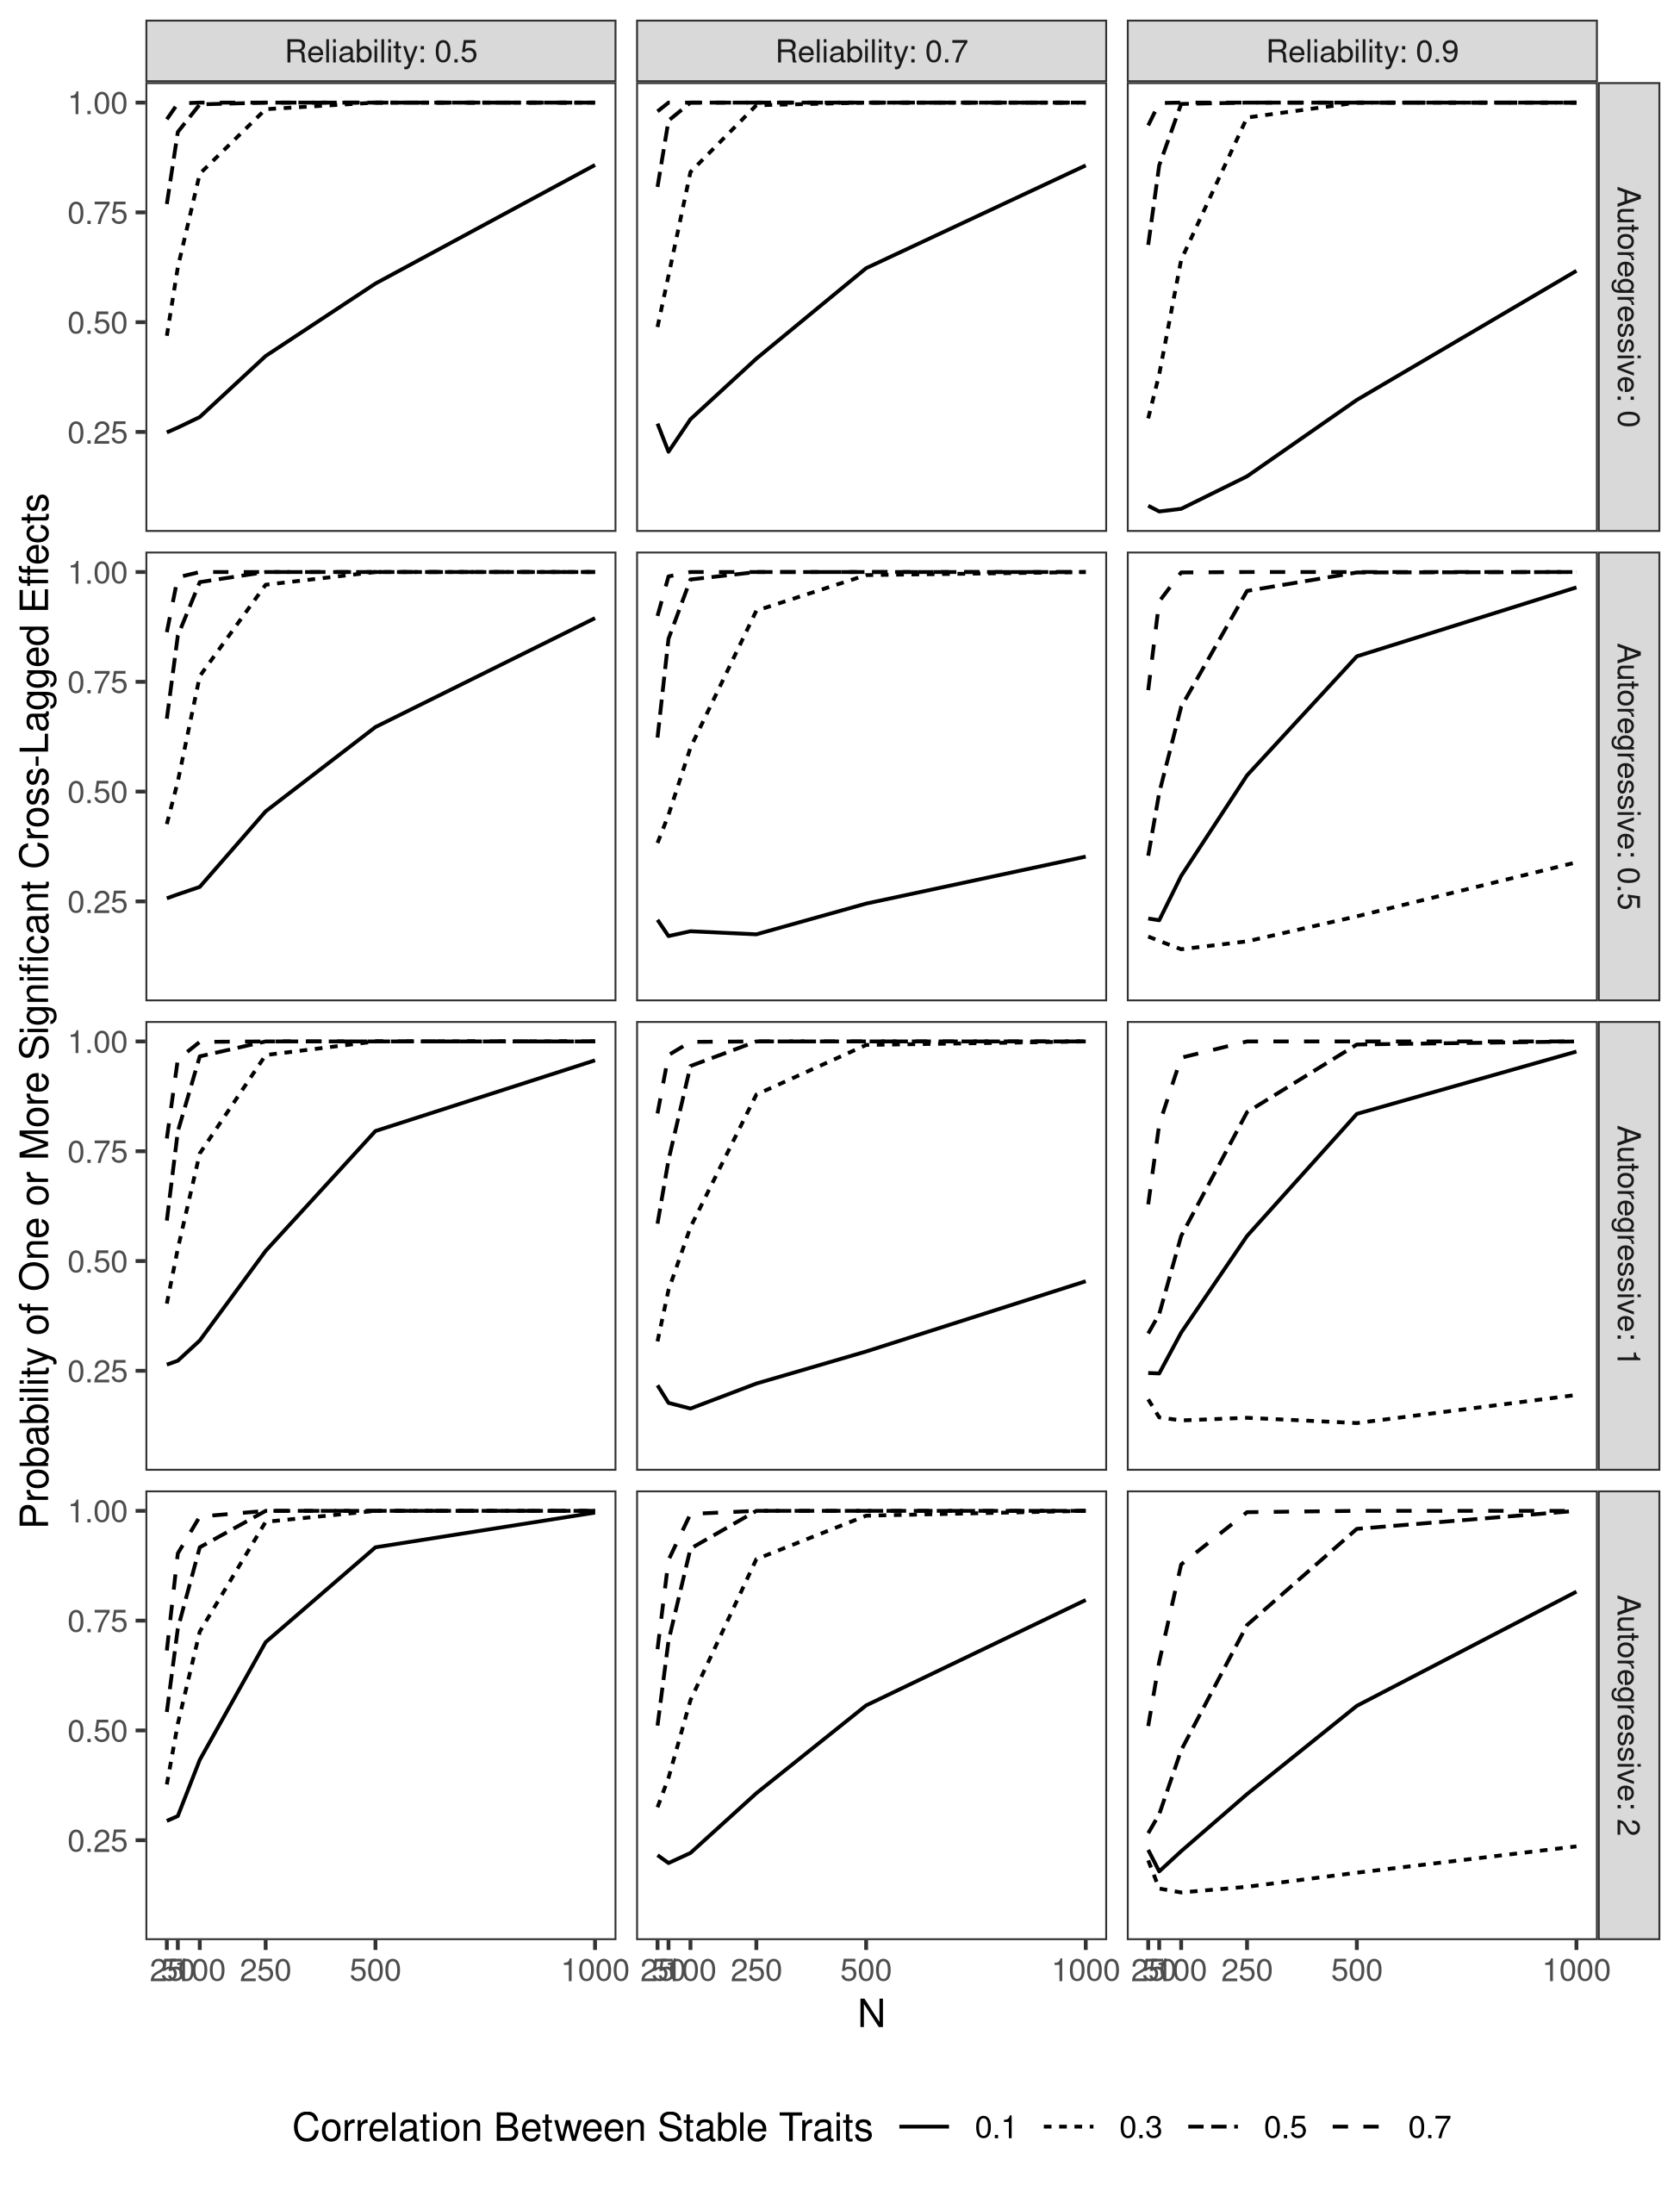
\includegraphics[width=6.5in,height=0.9\textheight]{images/10WaveSimulation} \caption{Simulation results for ten-wave CLPM. Columns reflect different reliabilities. Rows reflect different ratios of autoregressive to stabler-trait variance. Lines reflect different correlations between stable-trait components.}\label{fig:simFig10}
\end{figure}

\hypertarget{two-final-observations}{%
\subsection{Two Final Observations}\label{two-final-observations}}

The examples above focused almost entirely on cases where spurious effects were found when there were no cross-lagged paths in the data-generating model. However, failure to model associations between stable-trait components can also lead to the \emph{underestimation} of real cross-lagged paths. For instance, we can use the Shiny App to specify a model with variances of 1 for the two stable traits and the two autoregressive components, and then specify stabilities of .5 for X and Y and correlations of .5 for both the random intercepts and the initial autoregressive components. If we simulate data with cross lagged paths of .5 from X to Y and .2 from Y to X, the RI-CLPM reproduces these effects perfectly. However, even with no measurement error, the estimates from the CLPM are half the size that they should be. So the RI-CLPM is not necessarily more conservative than the CLPM when testing cross-lagged effects. Of course, everyone knows that an incorrect model will not provide accurate estimates; but my point is that most variables that psychologists study likely have at least some stable-trait-like variance, and ignoring it can have important consequences for the results that are obtained.

Finally, most of the simulations described above set the variance components, stabilities, and reliabilities to be equal across the X and Y variables. Yet researchers often have predictions about which variables have causal priority. If these structural features differ---for instance if the measures of X are more reliable than the measures of Y, or the autoregressive part of X is more stable than the autoregressive part of Y---then this can lead to evidence that one variable has causal priority over the other. I won't go into detail about these effects as others have discussed them and because the Shiny App is available to play around with. But researchers often report support for the causal priority of one variable using data from a CLPM, and subtle differences in these structural and psychometric properties can lead to important differences.

\hypertarget{wrapping-up}{%
\subsection{Wrapping Up}\label{wrapping-up}}

After describing the various approaches available to model longitudinal data, Orth et al. (2021) made the following recommendation: ``Before selecting a model, researchers should carefully consider the psychological or developmental process they would like to examine in their research, and then select a model that best estimates that process.'' This sounds like advice with which no one could argue. But if there is a plausible alternative model that describes the data as well as (or better than) the preferred model, then much more work is needed to defend that selection.

As an obvious example, if the true causal process linking self-esteem to depression was that changes in self-esteem instantaneously caused a corresponding change in depression (and there were no confounding factors), then that causal effect would be perfectly captured by the cross-sectional correlation between the two variables. Indeed, it would actually be problematic to rely on the cross-lagged association between self-esteem and depression controlling for earlier levels of depression as an estimate of the causal effect, because that would be conditioning on a collider. Yet few would find a cross-sectional correlation between self-esteem and depression to be compelling evidence for a causal effect of self-esteem precisely because there are so many plausible alternative possibilities.

The constructs that psychologists study very rarely have a purely autoregressive structure. At some point, the long-term stabilities of most constructs are stronger than would be suggested by the short-term stabilities and the length of time that has elapsed alone. This is likely due to the fact that many constructs have at least some stable-trait variance. And if there is stable trait variance, it is quite plausible that two constructs correlate at the stable-trait level. The simulations describe above show that it is quite easy to find cross-lagged effects in the presence of correlated stable traits (especially when there is measurement error), and the RI-CLPM and STARTS models provide a way to test this compelling and plausible alternative model.

\hypertarget{references}{%
\section*{References}\label{references}}
\addcontentsline{toc}{section}{References}

\hypertarget{refs}{}
\begin{CSLReferences}{1}{0}
\leavevmode\vadjust pre{\hypertarget{ref-cole_empirical_2005}{}}%
Cole, D. A., Martin, N. C., \& Steiger, J. H. (2005). Empirical and {Conceptual Problems With Longitudinal Trait-State Models}: {Introducing} a {Trait-State-Occasion Model}. \emph{Psychological Methods}, \emph{10}(1), 3--20. \url{https://doi.org/10.1037/1082-989x.10.1.3}

\leavevmode\vadjust pre{\hypertarget{ref-curran_separation_2014}{}}%
Curran, P. J., Howard, A. L., Bainter, S. A., Lane, S. T., \& McGinley, J. S. (2014). The separation of between-person and within-person components of individual change over time: {A} latent curve model with structured residuals. \emph{Journal of Consulting and Clinical Psychology}, \emph{82}(5), 879--894. \url{https://doi.org/10.1037/a0035297}

\leavevmode\vadjust pre{\hypertarget{ref-enders2007centering}{}}%
Enders, C. K., \& Tofighi, D. (2007). Centering predictor variables in cross-sectional multilevel models: {A} new look at an old issue. \emph{Psychological Methods}, \emph{12}(2), 121.

\leavevmode\vadjust pre{\hypertarget{ref-hamaker_critique_2015}{}}%
Hamaker, E. L., Kuiper, R. M., \& Grasman, R. P. P. P. (2015). A critique of the cross-lagged panel model. \emph{Psychological Methods}, \emph{20}(1), 102--116. \url{https://doi.org/f67cvh}

\leavevmode\vadjust pre{\hypertarget{ref-kenny_trait_1995}{}}%
Kenny, D. A., \& Zautra, A. (1995). The trait-state-error model for multiwave data. \emph{Journal of Consulting and Clinical Psychology}, \emph{63}(1), 52--59. \url{https://doi.org/10.1037/0022-006X.63.1.52}

\leavevmode\vadjust pre{\hypertarget{ref-Kenny2001}{}}%
Kenny, D. A., \& Zautra, A. (2001). The trait-state models for longitudinal data. In L. M. Collins \& A. G. Sayer (Eds.), \emph{New {Methods} for the {Analysis} of {Change}} (pp. 243--263). {Washington, DC}: {American Psychological Association}.

\leavevmode\vadjust pre{\hypertarget{ref-LucasInPressSIR}{}}%
Lucas, R. E., \& Donnellan, M. B. (2012). Estimating the {Reliability} of {Single-Item Life Satisfaction Measures}: {Results} from {Four National Panel Studies}. \emph{Social Indicators Research}, \emph{3}, 323--331.

\leavevmode\vadjust pre{\hypertarget{ref-ludtke_critique_2021}{}}%
Lüdtke, O., \& Robitzsch, A. (2021). A {Critique} of the {Random Intercept Cross-Lagged Panel Model}. {PsyArXiv}. \url{https://doi.org/10.31234/osf.io/6f85c}

\leavevmode\vadjust pre{\hypertarget{ref-orth_testing_2021}{}}%
Orth, U., Clark, D. A., Donnellan, M. B., \& Robins, R. W. (2021). Testing prospective effects in longitudinal research: {Comparing} seven competing cross-lagged models. \emph{Journal of Personality and Social Psychology}, \emph{120}(4), 1013--1034. \url{https://doi.org/gg7zfw}

\leavevmode\vadjust pre{\hypertarget{ref-usami_within-person_2021}{}}%
Usami, S. (2021). Within-{Person Variability Score-Based Causal Inference}: {A Two-Step Estimation} for {Joint Effects} of {Time-Varying Treatments}. \emph{arXiv:2007.03973 {[}Stat{]}}. Retrieved from \url{https://arxiv.org/abs/2007.03973}

\leavevmode\vadjust pre{\hypertarget{ref-usami_unified_2019}{}}%
Usami, S., Murayama, K., \& Hamaker, E. L. (2019). A unified framework of longitudinal models to examine reciprocal relations. \emph{Psychological Methods}, \emph{24}(5), 637--657. \url{https://doi.org/gf4fqx}

\leavevmode\vadjust pre{\hypertarget{ref-westfall_statistically_2016}{}}%
Westfall, J., \& Yarkoni, T. (2016). Statistically {Controlling} for {Confounding Constructs Is Harder} than {You Think}. \emph{PLOS ONE}, \emph{11}(3), e0152719. \url{https://doi.org/10.1371/journal.pone.0152719}

\end{CSLReferences}


\end{document}
